\documentclass[a4paper, 12pt]{article}
\usepackage[T2A]{fontenc} 
\usepackage[utf8]{inputenc}
\usepackage[english,russian]{babel} 


\usepackage{amsmath,amsfonts,amssymb,amsthm,mathtools}

\usepackage[left=2cm,right=2cm,top=2cm,bottom=2cm,bindingoffset=0cm]{geometry}
\usepackage{graphicx}

\newtheorem*{theorem}{Теорема}
\newtheorem*{corollary}{Следствие}
\newenvironment{Proof}
{\par\noindent{$\blacklozenge$}}
{\hfill$\scriptstyle\boxtimes$}

\usepackage[normalem]{ulem}
\usepackage[unicode]{hyperref}

%доп команды
\renewcommand{\mod}{\operatorname{mod}}
\newcommand{\rank}{\operatorname{rank}}
\newcommand{\tr}{\operatorname{tr}}
\newcommand{\pr}{\operatorname{\text{пр}}}
\renewcommand{\Im}{\operatorname{Im}}
\renewcommand{\Re}{\operatorname{Re}}
\renewcommand{\ker}{\operatorname{ker}}
\newcommand{\N}{\mathbb{N}}
\newcommand{\Z}{\mathbb{Z}}

%Красивые греческие буквы
\usepackage{upgreek}
\renewcommand{\alpha}{\upalpha}
\renewcommand{\beta}{\upbeta}
\renewcommand{\gamma}{\upgamma}
\renewcommand{\delta}{\updelta}
\renewcommand{\varphi}{\upvarphi}
\renewcommand{\epsilon}{\upepsilon}
\renewcommand{\psi}{\uppsi}


\title{\vspace{6.5cm}\textbf{\Huge{Алгебра и Теория чисел}}\\Конспект по 2 семестру 
	специальности «прикладная информатика»\\(лектор Г. В. Матвеев)}
\date{}
\begin{document}
	\maketitle
	\newpage
	\tableofcontents{}
	\newpage
\section{Прямая сумма подпространств}
Пусть $W_1$, $W_2$ --- подпространства.\\\\
$\bullet$ \textit{$W_1 \oplus W_2$ --- сумма называется \textbf{прямой}, если $W_1 \cap W_2 = \vec0$}.\\\\
Справедливо и следующее: $W_1 \oplus W_2 \oplus ... \oplus W_k$ называется прямой, если $W_i \cap \sum\limits_{i \neq j} W_j = \vec 0$
\begin{theorem}
    $$\dim(W_1 \oplus W_2) = \dim W_1 + \dim W_2$$
\end{theorem}
\begin{Proof}
    По теореме о сумме подпространств $$\dim(W_1+W_2)=\dim W_1+\dim W_2-\dim(W_1 \cap W_2)$$
    А так как $W_1 \cap W_2 = \vec0$, то $\dim(W_1 \cap W_2)=0$.
\end{Proof}
\begin{corollary}
	$$\dim(W_1 \oplus W_2 \oplus \ldots \oplus W_k) = \dim W_1 + \dim W_2 + \ldots + \dim W_k$$
\end{corollary}
\begin{theorem}
    Если $W \subset V_n \Rightarrow V_n = W \oplus U$, где $U$ --- подпространство.
\end{theorem} 
\begin{Proof}
    \begin{enumerate}
        \item $W = \vec0 \Rightarrow U = V_n$, $V_n = \vec0 \oplus V_n$
        \item $W = V_n \Rightarrow U = \vec0$, $V_n = V_n + \vec0$\\
        Оба равенства справедливы, так как $\vec0 \cap V_n = \vec0$
        \item Рассмотрим нетривиальный случай:
        $$W = L(v_1, v_2,...,v_r), \quad 0<r<n$$
        $$U = L(v_{r+1},v_{r+2},...,v_n)$$
        Возьмем произвольный вектор $x$, не нарушая общности:
        $$x=(\alpha_1v_1+...+\alpha_rv_r)+(\alpha_{r+1}v_{r+1}+...+\alpha_nv_n) \Rightarrow x=W+U$$
        Докажем, что $W \cap U = \vec0$.\\
        Пусть $x \in W \cap U$.
        $$x=\alpha_1v_1+...+\alpha_rv_r=\alpha_{r+1}v_{r+1}+...+\alpha_nv_n \Rightarrow \forall \alpha_i = 0 \Rightarrow x = 0 \Rightarrow W \cap U = \vec0$$
    \end{enumerate}
\end{Proof}
\begin{corollary}
	Каждое пространство раскладывается в прямую сумму $n$ одномерных подпространств.
	$$V_n=L(e_1) \oplus L(e_2) \oplus ... \oplus L(e_n)$$ 
\end{corollary}
$e_1,e_2, ... ,e_n$-базис.\\
То есть любой вектор раскладываетя по базису:
$$x=\alpha_1e_1+\alpha_2e_2+ ... + \alpha_ne_n$$

\section{Критерий совместности системы линейных уравнений}
\begin{theorem}
	Система линейных алгебраических уравнений совместна тогда и только тогда, когда ранг матрицы коэффицентов равен рангу расширенной матрицы.
\end{theorem}
\begin{Proof}
	Рассмотрим систему алгебраических уравнений
   $$ \begin{cases}
        a_{11}x_1+a_{12}x_2+...+a_{1n}x_n=b_1\\
        a_{21}x_1+a_{22}x_2+...+a_{2n}x_n=b_2\\
        \dotfill\\
        a_{m1}x_1+a_{m2}x_2+...+a_{mn}x_n=b_m
    \end{cases}$$
    \begin{center}
    $A = \begin{pmatrix}
    a_{11} & a_{12} & \dots & a_{1n}\\
    a_{21} & a_{22} & \dots & a_{2n}\\
    \vdots & \vdots & \ddots & \vdots\\
    a_{m1} & a_{m2} & \dots & a_{mn}
    \end{pmatrix}$
    --- матрица коэффицентов $A$.\\
    \end{center}
    \begin{center}
     $\begin{pmatrix}
    a_{11} & a_{12} & \dots & a_{1n} & \vline & b_1\\
    a_{21} & a_{22} & \dots & a_{2n} & \vline & b_2\\
    \vdots & \vdots & \ddots & \vdots & \vline & \vdots\\
    a_{m1} & a_{m2} & \dots & a_{mn} & \vline & b_m
    \end{pmatrix} =
    \widetilde{A} = (A|B)$ --- расширенная матрица.   
    \end{center}
    Система совместна $\Leftrightarrow \rank A=\rank\widetilde{A}$. \\
    $\Rightarrow$ Пусть система совместна с решением $(j_1,j_2, \dots, j_n)$\\
    $$\begin{pmatrix}
    a_{11}\\
    a_{21}\\
    \vdots\\
    a_{n1}
    \end{pmatrix} \cdot j_1+
    \begin{pmatrix}
    a_{12}\\
    a_{22}\\
    \vdots\\
    a_{n2}
    \end{pmatrix} \cdot j_2
    + \dots +
    \begin{pmatrix}
    a_{1n}\\
    a_{2n}\\
    \vdots\\
    a_{nn}
    \end{pmatrix} \cdot j_n = 
    \begin{pmatrix}
    b_1\\
    b_2\\
    \vdots\\
    b_n
    \end{pmatrix} \eqno (1)$$
    Это значит, что при добавлении столбца свободных членов базис не изменился, так как новый столбец выражается через старый. Следовательно, $\rank A=\rank\widetilde{A}$.\\\\
    $\Leftarrow$ Базисный минор  матрицы $A$ есть базисный минор матрицы $\widetilde{A}$, так как $rankA=rank\widetilde{A}$. Следовательно, столбец свободных членов 
    $ \begin{pmatrix}
    b_1\\
    b_2\\
    \vdots\\
    b_n
    \end{pmatrix}$ выражается через базисные столбцы по принципу (1). Коэффиценты остальных столбцов равны 0. И тогда полученные коэффиценты будут являться решением системы.
\end{Proof}

\subsection*{Решение системы линейных алгебраических уравнений с помощью критерия}
\begin{enumerate}
    \item Нахождение базисного минора матрицы $A$ методом окаймления минора.
    \item Проверяем условие $\rank A=\rank\widetilde{A}$ методом окаймления миноров.
    \item Отбрасываем все небазисные строки.
    \item Базисные неизвестные оставляем слева, а свободные переносим вправо.
\end{enumerate}

   $$ \begin{cases}
    a_{11}x_1+a_{12}x_2+ \dots + a_{1r}x_r = b_1-a_{1, r+1}x_{r+1}- \dots -a_{1n}x_n\\
    \dotfill\\
    a_{n1}x_1+a_{n2}x_2+ \dots + a_{nr}x_r = b_n-a_{n, r+1}x_{r+1}- \dots -a_{nn}x_n
    \end{cases}$$

Полученную систему рассматриваем как крамеровскую.\\
$$M=
\begin{vmatrix}
a_{11} & \dots & a_{1r}\\
\dots & \ddots & \dots\\
a_{r1} & \dots & a_{rr}
\end{vmatrix} \neq 0$$\\
\begin{equation*}
    \begin{cases}
    $$x_1=f_1(x_{r+1},\dots,x_n)$$\\
    \dotfill\\
    $$x_r=f_r(x_{r+1},\dots,x_n)$$
    \end{cases}
\end{equation*}
\section{Однородные системы линейных уравнений}
Рассмотрим однородную систему линейных уравнений
    $$\begin{cases}
    a_{11}x_1+a_{12}x_2+\dots+a_{1n}x_n=0,\\
    a_{21}x_1+a_{22}x_2+\dots+a_{2n}x_n=0\\
    \dotfill\\
    a_{m1}x_1+a_{m2}x_2+\dots+a_{mn}x_n=0
    \end{cases}\eqno(1)$$
Где
 $A=
\begin{pmatrix}
a_{11} & a_{12} & \dots & a_{1n}\\
a_{21} & a_{22} & \dots & a_{2n}\\
\vdots & \vdots & \ddots & \vdots\\
a_{m1} & a_{m2} & \dots & a_{mn}
\end{pmatrix}$ --- матрица системы,
$X=
\begin{pmatrix}
x_1\\
x_2\\
\vdots\\
x_n
\end{pmatrix}
$ --- столбец неизвестных.\\
\begin{center}
$0=
\begin{pmatrix}
0\\
0\\
\vdots\\
0
\end{pmatrix}$ --- столбец нулей.
\end{center}
Тогда систему (1) можно записать в матричном виде как
$$\textbf{AX=0}$$
\begin{theorem}
    Решения однородной системы линейных уравнений образуют векторное пространство, размерность которого $\dim W=n-r$ ($n$ --- число неизвестных, $r$ --- ранг системы, $r=\rank A=\rank(A|0)$.
\end{theorem}
\begin{Proof}
   Докажем, что это пространство. Вспомним необходимые критерии:
   $$W_1, W_2  \in W \Rightarrow W_1+W_2 \in W$$
   $$W_1 \in W \Rightarrow \lambda W_1 \in W$$
   Пусть $X_1$ --- конкретный набор, $X_1=
\begin{pmatrix}
x_1\prime\\
x_2\prime\\
\vdots\\
x_n\prime
\end{pmatrix}$. Тогда выполняются свойства
$$AX_1=0,\ AX_2=0 \Rightarrow A(X_1+X_2)=0$$
$$AX_1=0 \Rightarrow \lambda AX_1=0$$
Перенесем свободные неизвестные в системе в левую сторону.
    $$\begin{cases}
    a_{11}x_1+a_{12}x_2+ \ldots + a_{1r}x_r = b_1-a_{1, r+1}x_{r+1}- \ldots -a_{1n}x_n\\
    \dotfill\\
    a_{m1}x_1+a_{m2}x_2+ \ldots + a_{mr}x_r = b_m-a_{m, r+1}x_{r+1}- \ldots -a_{mn}x_n
    \end{cases}\eqno(3)$$
Базисный минор для этой системы $$M=
\begin{vmatrix}
a_{11} & \dots & a_{1r}\\
\dots & \ddots & \dots\\
a_{r1} & \dots & a_{rr}
\end{vmatrix} \neq 0$$
Где неизвестные $x_1,\dots,x_r$ --- базисные, а
$x_{r+1},\dots,x_n$ --- свободные.\\
Выражаем базисные неизвестные через свободные по правилу Крамера или Гаусса:
\begin{equation*}
    \begin{cases}
    $$x_1=f_1(x_{r+1},\dots,x_n)$$\\
    \dotfill\\
    $$x_r=f_r(x_{r+1},\dots,x_n)$$
    \end{cases}
\end{equation*}
Найдем базисные решения. Для этого
передадим значения 
$$\begin{cases}
    c_1=(c_{11},c_{12},\dots,c_{1r},1,0,\dots,0)\\
    c_2=(c_{21},c_{22},\dots,c_{2r},0,1,\dots,0)\\
    \dotfill\\
    c_{n-r}=(c_{n-r,1},c_{n-r,2},\dots,c_{n-r,r},0,0,\dots,1)
\end{cases}$$
Переменные, которым были переданы значения 0 и 1, являются базисными. Векторы являются линейно независимыми благодаря этим переменным.\\\\
Докажем, что любое решение выражается через базис.
$$(\gamma_1,\dots,\gamma_r,\gamma_{r+1},\dots,\gamma_n)-\gamma_{r+1}c_1-\ldots-\gamma_nc_{n-r}=(\gamma_1c_1,\gamma_2c_2,\dots,\gamma_nc_{n-r})$$
Значит все решения выражаются через базис.
\end{Proof}\\\\
$\bullet$ \textit{Базисные решения ОСЛУ называются \textbf{фундаментальной системой решений}.}
\subsection*{Решение неоднородной системы через однородную}
Будем обозначать $AX=B$ --- \textbf{неоднородная система}, $AY=0$ --- \textbf{однородная система}.
$$\left.
  \begin{array}{ccc}
    AX=B \\
    AY=0 \\
  \end{array}
\right\}=A(X+Y)=AX+AY=B+0=B$$
\begin{enumerate}
    \item Разность 2-ух решений неоднородной системы будет решением однородной.
    \item Если от решения неоднородной системы отнять фиксированное решение неоднородной системы, то получится решение однородной системы.
    $$AX-AX_0=B-B=0$$
    \item Произвольное решение неоднородной системы можно получить, добавляя к фиксированному решению некоторые решения однородной системы.
\end{enumerate}
\section{Линейные преобразования векторных пространств}
$\bullet$ \textit{Отображение $\varphi: V \rightarrow V$ (само в себя) называется \textbf{линейным}, если}
\begin{enumerate}
    \item \textit{Образ суммы равен сумме образов:}
    $$\varphi(a+b)=\varphi(a)+\varphi(b)$$
    \item \textit{При умножении вектора на скаляр его образ умножается на этот же скаляр:}
    $$\varphi(\lambda a)=\lambda \varphi(a)$$
\end{enumerate}
Если $\varphi: V \rightarrow W$, то $\varphi$ --- линейное отображение.\\\\
\textit{\textbf{Свойства линейного преобразования:}}
\begin{enumerate}
    \item \textit{Образ линейной комбинации равен такой же линейной комбинации образов (под действием линейного преобразования)}
    $$\varphi(\lambda_1a_1+\lambda_2a_2+\dots+\lambda_na_n=\lambda_1\varphi(a_1)+\lambda_2\varphi(a_2)+\dots+\lambda_n\varphi(a_n)$$
    \item \textit{Преобразование} $\vec0$
    $$\varphi(\vec0)=\vec0$$
    $$\varphi(\vec0)=\varphi(\vec0\cdot\vec a)=0\cdot \varphi(\vec a)=\vec0$$
    \item \textit{Вынесение минуса}
    $$\varphi(-\vec a)=-\varphi(\vec a)$$
    \item \textit{Линейное преобразование переводит линейно зависимые векторы в линейно зависимые с такими же скалярами.}
\end{enumerate}
\begin{theorem}
    Любое линейное преобразование вполне определяется своими значениями на базисных векторах и эти значения могут быть любыми.
\end{theorem}
    \begin{Proof}
       Пусть $e_1,e_2,\dots,e_n$ --- базис, $a_1,a_2,\dots,a_n$ --- системы векторов.\\
       Возьмем функцию $\varphi$ такую, что:
       \begin{equation*}
           \begin{cases}
                  $$\varphi(e_1)=a_1$$\\
                  $$\varphi(e_2)=a_2$$\\
                  \dotfill\\
                  $$\varphi(e_n)=a_n$$
           \end{cases}
       \end{equation*}
       Докажем, что такое пространство существует:
       $$x=x_1e_1+x_2e_2+\dots+x_ne_n$$
       $$\varphi(x)=x_1a_1+x_2a_2+\dots+x_na_n$$
       Докажем, что оно линейное:
       $$y=y_1e_1+y_2e_2+\dots+y_ne_n$$
       \begin{itemize}
           \item $\varphi(x+y)=(x_1+y_1)a_1+(x_2+y_2)a_2+\ldots+(x_n+y_n)a_n=x_1a_1+y_1a_1+\ldots+x_na_n+y_na_n=(x_1a_1+x_2a_2+\ldots+x_na_n)+(y_1a_1+y_2a_2+\ldots+y_na_n)=\varphi(x)+\varphi(y);$
           \item $\varphi(\lambda x)=\lambda x_1a_1+\lambda x_2a_2+\ldots+\lambda x_na_n = \lambda \varphi(x).$
       \end{itemize}
       Докажем, что единственное:\\
       Пусть существует 
       \begin{equation*}
       \begin{cases}
              $$\psi(e_1)=a_1$$\\
              $$\psi(e_2)=a_2$$\\
              \dotfill\\
              $$\psi(e_n)=a_n$$
       \end{cases}    
       \end{equation*} с такими же свойствами. Тогда
       $$\psi(x)=\psi(x_1e_1+x_2e_2+\dots+x_ne_n)=x_1\psi(e1)+x_2\psi(e_2)+\dots+x_n\psi(e_n)=x_1a_1+x_2a_2+\dots+x_na_n=\varphi(x)$$
    \end{Proof}

\section{Операции над линейными преобразованиями}
Пусть $f, \varphi$ --- линейные преобразования векторного пространства $V$.
\begin{enumerate}
    \item \textbf{Сумма линейных преобразований:} $$f(x) + \varphi(x) = (f+\varphi)(x),\ \forall x \in V.$$
    \begin{Proof}
    	$(f+\varphi)(\lambda_1 x_1 + \lambda_2 x_2)=f(\lambda_1 x_1 + \lambda_2 x_2) + \varphi(\lambda_1 x_1 + \lambda_2 x_2)=f(\lambda_1 x_1) + f(\lambda_2 x_2) + \varphi(\lambda_1 x_1) + \varphi(\lambda_2 x_2) = \lambda_1f(x_1)+\lambda_2f(x_2)+\lambda_1\varphi(x_1)+\lambda_2\varphi(x_2)=\lambda_1(f(x_1)+\varphi(x_1))+\lambda_2(f(x_2)+\varphi(x_2))=\lambda_1(f+\varphi)(x_1)+\lambda_2(f+\varphi)(x_2)$.
    \end{Proof} 
    \item \textbf{Умножение на скаляр линейного преобразования:} $$(\lambda f)(x) =  \lambda f(x),\ \forall x \in V.$$
    \begin{Proof}
    	$(\lambda f)(\lambda_1 x_1 + \lambda_2 x_2)=(\lambda f)(\lambda_1 x_1)+(\lambda f)(\lambda_2 x_2)=\lambda f(\lambda_1 x_1)+\lambda f(\lambda_2 x_2)=\lambda(f(\lambda_1 x_1)+\lambda(f(\lambda_2 x_2))=\lambda f(\lambda_1x_1+\lambda_2x_2)$.
    \end{Proof} 
    \item \textbf{Композиция линейных преобразований:} $$(f\circ \varphi)(x) = f(\varphi(x)),\ \forall x \in V.$$
    \begin{Proof}
    	$(f\varphi)(\lambda_1x_1+\lambda_2x_2)=f(\varphi(\lambda_1x_1+\lambda_2x_2))=f(\varphi(\lambda_1x_1)+\varphi(\lambda_2x_2))=f)\lambda_1\varphi(x_1)+\lambda_2\varphi(x_2))=\lambda_1f(\varphi(x_1))+\lambda_2f(\varphi(x_2))=\lambda_1(f\varphi)(x_1)+\lambda_2(f\varphi)(x_2)$.
    \end{Proof} 
\end{enumerate}
\section{Ядро и образ линейного преобразования}
Пусть $\varphi:V\rightarrow V$ --- линейное преобразование.\\\\
$\bullet$ \textit{Множество $\ker \varphi = \{x\ |\ \varphi(x)=\vec 0\}$ --- \textbf{ядро} линейного преобразования.}\\
$\dim \ker \varphi$ - \textbf{дефект} линейного преобразования (размерность ядра).\\\\
$\bullet$ \textit{Множество $\Im \varphi = \varphi(v)=\{\varphi(x)\ |\ x \in V\}$ --- \textbf{образ} линейного преобразования.}\\
$\dim \Im \varphi$ - \textbf{ранг} линейного преобразования (размерность образа).\\\\
\textbf{Пример 1}\\
Рассмотрим функцию $\sin(x)$. Функция синуса не является линейной, в чем легко убедиться ($\sin(a+b) \neq \sin a + \sin b$), однако для нее можно определить ядро и образ. Таким образом
$$\ker (\sin) = {\pi n}$$
$$\Im (\sin) = [-1,1]$$
\textbf{Пример 2}\\
Тождественное преобразование - $\varphi(v)=v \quad \forall v \in V$
$$\ker( \varphi) = \vec 0$$
$$\Im (\varphi) = V$$
\textbf{Пример 3}\\
Возьмем прямую $l$ и плоскость $P$, где $l \perp P$.
\begin{figure}[h]
    \begin{center}
    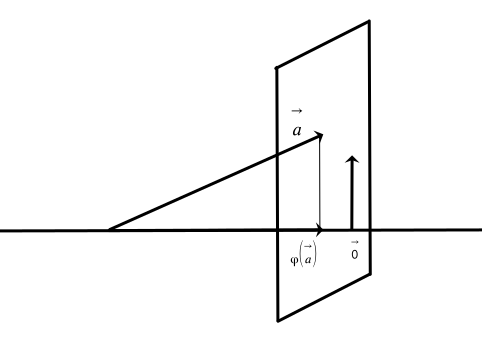
\includegraphics[scale=0.8]{0st25sYXFU (1).png}
    \end{center}
    \end{figure}\\
$$\varphi(\vec a)=\vec pr a$$
$$\Im (\varphi) = l = V_1$$
$$\ker (\varphi) = P = V_2$$
\begin{theorem}
    Ядро и образ линейного преобразования --- подпространства исходного векторного пространства.
\end{theorem}
\begin{Proof}
	Проверим выполнимость свойств:
   \begin{enumerate}
       \item $w_1,w_2 \in \ker (\varphi) \Rightarrow \varphi(w_1)=\varphi(w_2)=\vec 0$
       $\varphi(w_1+w_2)=\varphi(w_1)+\varphi(w_2)=\vec 0+ \vec 0=\vec 0 \Rightarrow w_1+w_2 \in \ker (\varphi)$
       \item $\lambda \varphi(w)=\lambda \vec 0=\vec 0 \Rightarrow \lambda \varphi \in \ker (\varphi)$
       \item $\varphi(w_1),\varphi(w_2) \in \Im (\varphi)$\\
       $\varphi(w_1)+\varphi(w_2)=\varphi(w_1+w_2) \in \Im (\varphi)$
       \item $\lambda \varphi(w_1)=\varphi(\lambda w_1) \in \Im (\varphi)$
   \end{enumerate}
\end{Proof}\\
$\bullet$ \textit{Размерность ядра --- \textbf{дефект}. Будем обозначать} $d = \dim( \ker (\varphi))$.\\\\
$\bullet$ \textit{Размерность образа --- \textbf{ранг}. Будем обозначать} $r = \rank \varphi = \dim  (\Im (\varphi))$.\\\\
Тогда $\varphi$ --- \textbf{нулевое преобразование}, если $d=n$, $r=0$.\\
$\varphi$ --- \textbf{тождественное преобразование}, если $d=0$, $r=n$.\\
$\varphi$ --- \textbf{проектирование векторов}, если $d=2$, $r=1$.
\begin{theorem}
    Сумма ранга и дефекта равняется размерности пространства.
\end{theorem}
\begin{Proof}
   Рассмотрим образ $\varphi(V)$. Пусть базис $\varphi(V):\varphi(\varphi(l_1),\varphi(l_2),\dots,\varphi(l_r))$\\
   Докажем, что $$V_n=L(l_1,l_2,\dots,l_r) \oplus \ker(\varphi)$$
   $$n=r+d$$
   \begin{enumerate}
       \item $l_1,l_2,\dots,l_r$ --- линейно независимы.\\
       По свойству линейное преобразование сохраняет зависимость. Если бы $l_1,l_2,\dots,l_r$ были зависимы, то и $\varphi(l_1),\varphi(l_2),\dots,\varphi(l_r)$ были бы зависимы, но это базис, значит не зависимы.
       \item $\vec v \in V_n = \vec x \in L(l_1,l_2,\dots,l_r) + \vec y \in ker \varphi$\\
       $$\varphi(V) = \alpha_1\varphi(l_1)+\alpha_2\varphi(l_2)+\\dots+\alpha_r\varphi(l_r)$$
       $$\varphi(v-\alpha_1 l_1-\ldots-\alpha_r l_r)=\vec 0 \Rightarrow v-\alpha_1 l_1-\ldots-\alpha_r l_r = y \in \ker \varphi$$
       $$v = \alpha_1 l_1-\ldots-\alpha_r l_r + y = x + y$$
       \item $L \cap ker \varphi = \vec 0$\\
       Пусть $x \in L \cap \ker \varphi$.\\
       $x = \alpha_1 l_1+\ldots+\alpha_r l_r$\\
       $\varphi(x) = \vec 0, \quad \varphi(x) = \varphi(\alpha_1 l_1+\ldots+\alpha_r l_r) = \varphi(\alpha_1 l_1)+\varphi(\alpha_2 l_2)+\ldots+\varphi(\alpha_r l_r)=\alpha_1\varphi(l_1)+\alpha_2\varphi(l_2)+\ldots+\alpha_r\varphi(l_r) = \vec 0 \Rightarrow \alpha_1=\alpha_2=\ldots=\alpha_r=0 \Rightarrow x=\vec 0$
   \end{enumerate}
\end{Proof}

\section{Матрица линейного преобразования}
Пусть $V$ --- векторное пространство с базисом $e_1, e_2, \dots, e_n$.
$$x \in V, \quad x = x_1e_1+x_2e_2+\dots+x_ne_n$$
$\bullet$ Пусть $\varphi: V \rightarrow V$ --- \textbf{линейное преобразование} векторного пространства $V$.\\
Подействуем этим преобразованием поочередно на все базисные векторы и полученные векторы выразим через базис:
$$\begin{cases}
     \varphi(e_1)=\alpha_{11}e_1+\alpha_{21}e_2+\dots+\alpha_{n1}e_n\\  
     \varphi(e_2)=\alpha_{12}e_1+\alpha_{22}e_2+\dots+\alpha_{n2}e_n\\ 
     \dotfill\\
     \varphi(e_n)=\alpha_{1n}e_1+\alpha_{2n}e_2+\dots+\alpha_{nn}e_n\\ 
\end{cases}\eqno(1)$$
\begin{center}
Матрица $A = 
    \begin{pmatrix}
    \alpha_{11} & \alpha_{12} & \dots & \alpha_{1n}\\
    \alpha_{21} & \alpha_{22} & \dots & \alpha_{2n}\\
    \vdots & \vdots & \ddots & \vdots\\
    \alpha_{n1} & \alpha_{n2} & \dots & \alpha_{nn}
    \end{pmatrix}$ --- матрица линейного преобразования $\varphi$.
\end{center}
$\bullet$ Столбцами матрицы линейного преобразования являются координаты образов базисных векторов.\\\\
Рассмотрим пример:\\
На вектор $x = x_1e_1+x_2e_2+\dots+x_ne_n$ подействуем линейным преобразованием.
$$\varphi(x) = x_1\varphi(e_1)+x_2\varphi(e_2)+\ldots+x_n\varphi(e_n),$$
где $\varphi(e_1), \varphi(e_2), \dots, \varphi(e_n)$ --- столбцы матрицы $A$.\\
Тогда систему (1) можно переписать следующим образом:\\
Пусть $e = (e_1, e_2, \dots, e_n)$, тогда
$$(e_1, e_2, \dots, e_n)A=(\varphi(e_1), \varphi(e_2), \dots, \varphi(e_n))$$
$$\varphi(e)=eA$$
Вектор $x$ запишем как $x=eX$, где 
$X=
\begin{pmatrix}
x_1\\
x_2\\
\vdots\\
x_n
\end{pmatrix}$.
Тогда линейное преобразование вектора $x$ примет вид:
$$\varphi(x)=\varphi(e)X$$
$$\varphi(x)=eAX$$
Это говорит о том, что $X \xrightarrow{\varphi} AX \sim \varphi(X)=AX$.\\\\
\textbf{Теорема.}
    \begin{enumerate}
        \item \textit{При сложении линейных преобразований их матрицы в данном базисе складываются.}
        \item \textit{При умножении линейных преобразований их матрицы в данном базисе умножаются.}
        \item \textit{При умножении линейного преобразования на скаляр его матрица умножается на тот же скаляр.}
    \end{enumerate}

\begin{Proof}
Пусть $V$ --- векторное пространство с базисом $e_1, e_2, \dots, e_n$.\\
И пусть $f, \varphi$ --- линейные преобразования.\\
Подействовав этими линейными преобразованиями на базис $V$ получим следующие системы:
$$\begin{cases}
     f(e_1)=\alpha_{11}e_1+\alpha_{21}e_2+\dots+\alpha_{n1}e_n\\  
     f(e_2)=\alpha_{12}e_1+\alpha_{22}e_2+\dots+\alpha_{n2}e_n\\ 
     \dotfill\\
     f(e_n)=\alpha_{1n}e_1+\alpha_{2n}e_2+\dots+\alpha_{nn}e_n\\ 
\end{cases}\eqno(1)$$

$$\begin{cases}
     \varphi(e_1)=\beta_{11}e_1+\beta_{21}e_2+\dots+\beta_{n1}e_n\\  
     \varphi(e_2)=\beta_{12}e_1+\beta_{22}e_2+\dots+\beta_{n2}e_n\\ 
     \dotfill\\
     \varphi(e_n)=\beta_{1n}e_1+\beta_{2n}e_2+\dots+\beta_{nn}e_n\\ 
\end{cases}\eqno(2)$$\\
Запишем матрицы линейных преобразований для $f, \varphi$:\\
\begin{center}
$A = 
\begin{pmatrix}
\alpha_{11} & \alpha_{12} & \dots & \alpha_{1n}\\
\alpha_{21} & \alpha_{22} & \dots & \alpha_{2n}\\
\vdots & \vdots & \ddots & \vdots\\
\alpha_{n1} & \alpha_{n2} & \dots & \alpha_{nn}
\end{pmatrix}$ --- матрица линейного преобразования $f$.
\end{center}
\begin{center}
$B = 
\begin{pmatrix}
\beta_{11} & \beta_{12} & \dots & \beta_{1n}\\
\beta_{21} & \beta_{22} & \dots & \beta_{2n}\\
\vdots & \vdots & \ddots & \vdots\\
\beta_{n1} & \beta_{n2} & \dots & \beta_{nn}
\end{pmatrix}$ --- матрица линейного преобразования $\varphi$.
\end{center}
   \begin{enumerate}
       \item Сложим почленно строки систем (1) и (2).
        $$\begin{cases}
        f(e_1)+\varphi(e_1)=(\alpha_{11}+\beta_{11})e_1+(\alpha_{21}+\beta_{21})e_2+\dots+(\alpha_{n1}+\beta_{n1})e_n\\
        f(e_2)+\varphi(e_2)=(\alpha_{12}+\beta_{12})e_1+(\alpha_{22}+\beta_{22})e_2+\dots+(\alpha_{n2}+\beta_{n2})e_n\\
        \dotfill\\
        f(e_n)+\varphi(e_n)=(\alpha_{1n}+\beta_{1n})e_1+(\alpha_{2n}+\beta_{2n})e_2+\dots+(\alpha_{nn}+\beta_{nn})e_n\\ 
        \end{cases}$$
        Отсюда получим матрицу линейного преобразования $f+\varphi$:\\
        $$\begin{pmatrix}
        \alpha_{11}+\beta_{11} & \alpha_{12}+\beta_{12} & \dots & \alpha_{1n}+\beta_{1n}\\
        \alpha_{21}+\beta_{21} & \alpha_{22}+\beta_{22} & \dots & \alpha_{2n}+\beta_{2n}\\
        \vdots & \vdots & \ddots & \vdots\\
        \alpha_{n1}+\beta_{n1} & \alpha_{n2}+\beta_{n2} & \dots & \alpha_{nn}+\beta_{nn}\\
        \end{pmatrix} = A + B$$
        \item Будем рассматривать умножение линейных преобразований как компзицию отображений $\varphi(f(e))$.
        Подействуем линейным преобразованием $f$ на базисные векторы:
        $$\begin{cases}
        f(e_1)=\alpha_{11}e_1+\alpha_{21}e_2+\dots+\alpha_{n1}e_n\\  
        f(e_2)=\alpha_{12}e_1+\alpha_{22}e_2+\dots+\alpha_{n2}e_n\\ 
        \dotfill\\
        f(e_n)=\alpha_{1n}e_1+\alpha_{2n}e_2+\dots+\alpha_{nn}e_n\\ 
        \end{cases}\eqno(1)$$
        На полученные векторы подействуем линейным преобразованием $\varphi$:
        $$\begin{cases}
        \varphi(f(e_1))=\beta_{11}f(e_1)+\beta_{21}f(e_2)+\dots+\beta_{n1}f(e_n)\\  
        \varphi(f(e_2))=\beta_{12}f(e_2)+\beta_{22}f(e_2)+\dots+\beta_{n2}f(e_n)\\
        \varphi(f(e_n))=\beta_{1n}f(e_1)+\beta_{2n}f(e_2)+\dots+\beta_{nn}f(e_n)\\
        \end{cases}$$
        Подставим в полученную систему уравнения системы (1):\\\\
        $\begin{cases}
        \varphi(f(e_1))=\beta_{11}(\alpha_{11}e_1+\alpha_{21}e_2+\dots+\alpha_{n1}e_n)+\beta_{21}(\alpha_{12}e_1+\alpha_{22}e_2+\dots+\alpha_{n2}e_n)+\dots\\  
       \varphi(f(e_2))=\beta_{12}(\alpha_{11}e_1+\alpha_{21}e_2+\dots+\alpha_{n1}e_n)+\beta_{22}(\alpha_{12}e_1+\alpha_{22}e_2+\dots+\alpha_{n2}e_n)+\dots\\ 
        \varphi(f(e_n))=\beta_{1n}(\alpha_{11}e_1+\alpha_{21}e_2+\dots+\alpha_{n1}e_n)+\beta_{2n}(\alpha_{12}e_1+\alpha_{22}e_2+\dots+\alpha_{n2}e_n)+\dots\\ 
        \end{cases}$\\\\
        Раскроем скобки:\\\\
        $\begin{cases}
        \varphi(f(e_1))=\beta_{11}\alpha_{11}e_1+\beta_{11}\alpha_{21}e_2+\dots+\beta_{11}\alpha_{n1}e_n+\beta_{21}\alpha_{12}e_1+\beta_{21}\alpha_{22}e_2+\dots+\beta_{21}\alpha_{n2}e_n+\dots\\  
       \varphi(f(e_2))=\beta_{12}\alpha_{11}e_1+\beta_{12}\alpha_{21}e_2+\dots+\beta_{12}\alpha_{n1}e_n+\beta_{22}\alpha_{12}e_1+\beta_{22}\alpha_{22}e_2+\dots+\beta_{22}\alpha_{n2}e_n+\dots\\ 
        \varphi(f(e_n))=\beta_{1n}\alpha_{11}e_1+\beta_{1n}\alpha_{21}e_2+\dots+\beta_{1n}\alpha_{n1}e_n+\beta_{2n}\alpha_{12}e_1+\beta_{2n}\alpha_{22}e_2+\dots+\beta_{2n}\alpha_{n2}e_n+\dots\\ 
        \end{cases}$\\\\
        Сгрупируем подобные слагаемые:\\\\
        $\begin{cases}
        \varphi(f(e_1))=(\beta_{11}\alpha_{11}+\beta_{21}\alpha_{12}+\dots)e_1+(\beta_{11}\alpha_{21}+\beta_{21}\alpha_{22}+\dots)e_2+\dots\\  
       \varphi(f(e_2))=(\beta_{12}\alpha_{11}+\beta_{22}\alpha_{12}+\dots)e_1+(\beta_{12}\alpha_{21}+\beta_{22}\alpha_{22}+\dots)e_2+\dots\\ 
        \varphi(f(e_n))=(\beta_{1n}\alpha_{11}+\beta_{2n}\alpha_{12}+\dots)e_1+(\beta_{1n}\alpha_{21}+\beta_{2n}\alpha_{22}+\dots)e_2+\dots\\  
        \end{cases}$\\\\
        Запишем координаты векторов в матрицу линейного преобразования:\\\\
        $\begin{pmatrix}
        \beta_{11}\alpha_{11}+\beta_{21}\alpha_{12}+\dots & \beta_{12}\alpha_{11}+\beta_{22}\alpha_{12}+\dots & \dots & \beta_{1n}\alpha_{11}+\beta_{2n}\alpha_{12}+\dots\\
       \beta_{11}\alpha_{21}+\beta_{21}\alpha_{22}+\dots & \beta_{12}\alpha_{21}+\beta_{22}\alpha_{22}+\dots&\dots&
       \beta_{2n}\alpha_{21}+\beta_{2n}\alpha_{22}+\dots\\
        \vdots & \vdots & \ddots & \vdots\\
        \beta_{11}\alpha_{n1}+\beta_{21}\alpha_{n2}+\dots & \beta_{12}\alpha_{n1}+\beta_{22}\alpha_{n2}+\dots & \dots&
        \beta_{1n}\alpha_{n1}+\beta_{2n}\alpha_{n2}+\dots\\
        \end{pmatrix}=A\cdot B$
        \item Умножим каждую строку системы (1) на произвольный скаляр $\gamma$:
        $$\begin{cases}
        \gamma f(e_1)=\gamma\alpha_{11}e_1+\gamma \alpha_{21}e_2+\dots+\gamma \alpha_{n1}e_n\\  
        \gamma f(e_2)=\gamma \alpha_{12}e_1+\gamma \alpha_{22}e_2+\dots+\gamma \alpha_{n2}e_n\\ 
        \dotfill\\
        \gamma f(e_n)=\gamma \alpha_{1n}e_1+\gamma \alpha_{2n}e_2+\dots+\gamma \alpha_{nn}e_n\\ 
        \end{cases}$$
        Получаем матрицу линейного преобразования $\gamma f$:
        \begin{center}
        $\begin{pmatrix}
        \gamma \alpha_{11} & \gamma \alpha_{12} & \dots & \gamma \alpha_{1n}\\
        \gamma \alpha_{21} & \gamma \alpha_{22} & \dots & \gamma \alpha_{2n}\\
        \vdots & \vdots & \ddots & \vdots\\
        \gamma \alpha_{n1} & \gamma \alpha_{n2} & \dots & \gamma \alpha_{nn}
        \end{pmatrix} = \gamma A$
        \end{center}
   \end{enumerate}
\end{Proof}
\begin{theorem}
    Ранг линейного преобразования равен рангу его матрицы.
\end{theorem}
\begin{Proof}
$$\rank \varphi = \dim \varphi(V)$$
Так как образ есть \textit{линейная оболочка} $L(\varphi(e_1), \varphi(e_2), \dots, \varphi(e_n))$, то
$$\dim \varphi(V) = \dim L(\varphi(e_1), \varphi(e_2), \dots, \varphi(e_n)) = \rank(\varphi(e_1), \varphi(e_2), \dots, \varphi(e_n)) = \rank A$$
$$\rank \varphi = \rank A$$
\end{Proof}\\
\textbf{Пример 1}\\
$\varphi(x) = \vec 0, \quad \forall x$ --- нулевое преобразование.
$$\begin{cases}
     \varphi(e_1)=0e_1+0e_2+\dots+0e_n\\  
     \varphi(e_2)=0e_1+0e_2+\dots+0e_n\\ 
     \dotfill\\
     \varphi(e_n)=0e_1+0e_2+\dots+0e_n\\ 
\end{cases}$$
\begin{center}
    $A = \begin{pmatrix}
    0 & 0 & \dots & 0\\
    0 & 0 & \dots & 0\\
    \vdots & \vdots & \ddots & \vdots\\
    0 & 0 & \dots & 0
    \end{pmatrix}$
    --- матрица нулевого преобразования.\\
    \end{center}
\textbf{Пример 2}\\
$\varphi(x) = x, \quad \forall x$ --- тождественное преобразование.
$$\begin{cases}
     \varphi(e_1)=1e_1+0e_2+\dots+0e_n\\  
     \varphi(e_2)=0e_1+1e_2+\dots+0e_n\\ 
     \dotfill\\
     \varphi(e_n)=0e_1+0e_2+\dots+1e_n\\ 
\end{cases}$$
\begin{center}
    $A = \begin{pmatrix}
    1 & 0 & \dots & 0\\
    0 & 1 & \dots & 0\\
    \vdots & \vdots & \ddots & \vdots\\
    0 & 0 & \dots & 1
    \end{pmatrix}$
    --- матрица тождественного преобразования.\\
    \end{center}    
\textbf{Пример 3}
\begin{figure}[h]
    \begin{center}
    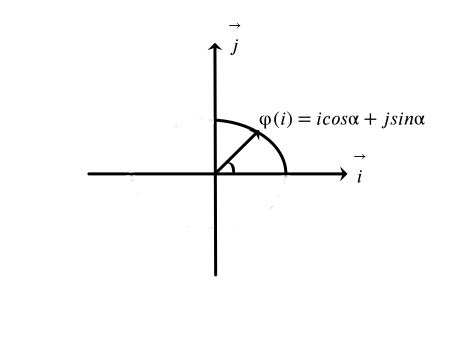
\includegraphics[scale=0.8]{2.png}
    \end{center}
    \end{figure}\\
\begin{center}
    $A = \begin{pmatrix}
    \cos \alpha & -\sin \alpha\\
    \sin \alpha & \cos \alpha\\
    \end{pmatrix}$
    --- матрица угла поворота системы координат на угол $\alpha$.\\
    \end{center}
    $\bullet$ \textit{Биективное (взаимооднозначное) линейное преобразование называется \textbf{автоморфизмом}.}\\\\
    Если $\varphi: V \rightarrow V$ --- линейное преобразование, то $\varphi$ --- автоморфизм $\Leftrightarrow$ $\varphi$ --- биекция.
    \begin{theorem}
        Линейное преобразование $\varphi$ --- автоморфизм $\Leftrightarrow$ его матрица невырожденная.
    \end{theorem}
    \begin{Proof}
    $$\varphi(X)=AX$$
    $\Rightarrow$ Предположим, что $|A| = 0$ (т.е. матрица вырожденная).\\
    Тогда $AX=0$ $\Rightarrow$ система уравнений линейного преобразования имеет несколько решений и ноль имеет несколько прообразов, чего быть не может.\\\\
    $\Leftarrow$ Имеем, что $|A| \neq 0$ (т.е. матрица невырожденная).\\
    Значит для $AX=B$ имеется только одно решение по правилу Крамера $\Rightarrow$ $\varphi$ --- биекция.
    \end{Proof}
    \section{Подобные матрицы}
    Для определения подобия матриц рассмотрим задачу.\\\\
    \textbf{Задача}\\
    Пусть $u, v$ --- некоторые базисы, $\varphi$ --- линейное преобразование. Применим его к обоим базисам:
    $$\varphi(u) = \varphi(u_1), \varphi(u_2), \dots, \varphi(u_n) = (u_1,u_2,\dots,u_n)A$$
    Запишем полученные преобразования в матричном виде:
    $$\varphi(u)=uA$$
    $$\varphi(v)=vB$$
    Пусть $S$ --- матрица перехода от базиса $u$ к базису $v$ ($|S| \neq 0$ --- матрица невырожденная), то есть $v=uS$.\\
    \textit{Найти}: связь между матрицами $A$ и $B$.\\
    \textit{Решение:}\\
    Подействуем линейным преобразованием $\varphi$ на $v=uS$:
    $$\varphi(v)=\varphi(u)S$$
    Подставим в это равенство значение $\varphi(u)$, полученное выше:
    $$\varphi(v)=uAS\eqno(1)$$
    Так как $\varphi(v) = vB$ и $v=uS$, то, подставив значение $v$ в первое уравнение, получим:
    $$\varphi(v)=uSB\eqno(2)$$
    Приравняем правые части уравнений (1) и (2):
    $$uAS=uSB$$
    $$u(SB-AS)=(\vec0,\vec0,\dots,\vec0)$$
    \textit{Так как векторы $u_1,u_2,\dots,u_n$ линейно независимы как базис и их линейные комбинации равны $\vec0$, то элементы матрицы $SB-AS$ равны 0 $\Rightarrow SB=AS \Rightarrow B=S^{-1}AS$.}\\\\
    $\bullet$ Матрицы $A$ и $B$, связанные соотношением $B=S^{-1}AS$, называются \textbf{подобными}.\\\\
    $\bullet$ Матрицы одного и того же преобразования в разных базисах \textbf{подобны}.\\\\
    $\bullet$ Если для матриц $A$ и $B$ справедливо равенство $B=S^{-1}AS$, то можно найти линейное преобразование и базисы, которые будут иметь эти матрицы.
    \begin{theorem}
        Две квадратных матрицы одного и того же порядка являются матрицами одного и того же преобразования $\Leftrightarrow$ они подобны.
    \end{theorem}
    \textbf{Свойства подобных матриц}
    \begin{enumerate}
        \item \textit{Всякая матрица подобна самой себе:}
        $$A=E^{-1}AE$$
        \item \textit{Подобие матриц транзитивно:}\\
        Возьмем матрицы $A, B, C$, связанные соотношением:
        $$C=T^{-1}BT$$
        $$B=S^{-1}AS$$
        Подставим значение $B$:
        $$C=T^{-1}S^{-1}AST$$
        Используя свойство обратных матриц
        $$T^{-1}S^{-1}=(ST)^{-1}$$
        и подставя полученное значение в предыдущее равенство, получаем:
        $$C=(ST)^{-1}A(ST)$$
        \item \textit{Подобие матриц симметрично:}
        $$A=T^{-1}BT \Leftrightarrow B=S^{-1}AS$$
        Рассмотрим равенство $B=S^{-1}AS$. Домножим левую и правую часть на $S^{-1}$ и $S$:
        $$A=SBS^{-1}$$
        Пусть $T=S^{-1} \Rightarrow T^{-1}=S$. Подставим это в равенство и получим:
        $$A=T^{-1}BT$$
        То есть если матрица $B$ подобна матрице $A$, то мы можем найти такую матрицу $T$, чтобы матрица $A$ была подобна матрице $B$.
        \item \textit{Определители подобных матриц равны:}
        $$|B|=|S^{-1}AS|=|S^{-1}|\cdot|A|\cdot|S|=|A|\cdot|S|\cdot|S^{-1}|=|A|\cdot|SS^{-1}|=|A|\cdot|E|=|A|\cdot1=|A|$$
        \item \textit{Ранги подобных матриц равны:}
        $$B=S^{-1}AS \Rightarrow \rank A = \rank B = \rank f$$
        Это объясняется тем, что ранг преобразования равен рангу матрицы:
        $$\rank A = \rank f, \quad \rank B = \rank f \Rightarrow \rank A = \rank B$$
    \end{enumerate}
    \section{Инвариантные подпространства}
    Пусть $\varphi: V \rightarrow V$ --- преобразование векторного пространства, $W$ -- подпространство.\\
    $W$ называется \textbf{инвариантным}, если $\varphi(W) \subset W$.\\\\
    \textbf{Примеры}
    \begin{enumerate}
        \item $\varphi(V) = V, \ \varphi = e$ --- все подпространства инвариантны.
        \item $W = \vec0, \ \varphi(\vec0) = \vec0$ --- нулевое подпространство всегда инвариантно.
        \item $W = V$ --- само пространство инвариантно.
        \item $\varphi(W) = 0 \in W, \ \varphi = 0$ --- нулевое преобразование.\\
        Все подпространства инвариантны.
        \item $\varphi = \lambda e$ --- скалярное преобразование.\\
        Все подпространства инвариантны.
        \item Проектирование в 3-х мерном пространстве на прямую:
        $$\varphi = \pr_l P$$
        \begin{figure}[h]
    \begin{center}
    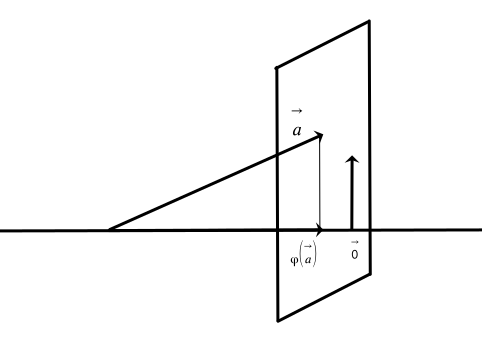
\includegraphics[scale=0.8]{0st25sYXFU (1).png}
    \end{center}
    \end{figure}\\
        Инвариантные подпространства:
        \begin{itemize}
            \item Все векторы прямой;
            \item Векторы, перпендикулярные плоскости.
        \end{itemize}
    \end{enumerate}
    \begin{theorem}
        Сумма и пересечение инвариантных пространств инвариантны.
    \end{theorem}
    \begin{Proof}
    Пусть $x = W_1 \cap W_2$.\\
    Так как $W_1$ --- инвариантно, то $\varphi(x) \in W_1$, аналогично для $W_2$.\\
    Так как $\varphi(x) \in W_1$ и $\varphi(x) \in W_2$, то $\varphi(x) \in W_1 \cap W_2 \Rightarrow W_1 \cap W_2$ --- инвариантно.\\\\
    Пусть $x \in W_1 + W_2 \Rightarrow x \in W_1$ или $x \in W_2$.\\
    Так как $W_1$ и $W_2$ --- инвариантны, то $\varphi(x) \in W_1$ или $\varphi(x) \in W_2 \Rightarrow \varphi(x) \in W_1 + W_2 \Rightarrow W_1 + W_2$ --- инвариантно.
    \end{Proof}\\\\\\
    $\bullet$ Матрица называется \textbf{полураспавшейся}, если она имеет вид
    \begin{figure}[h]
    \begin{center}
    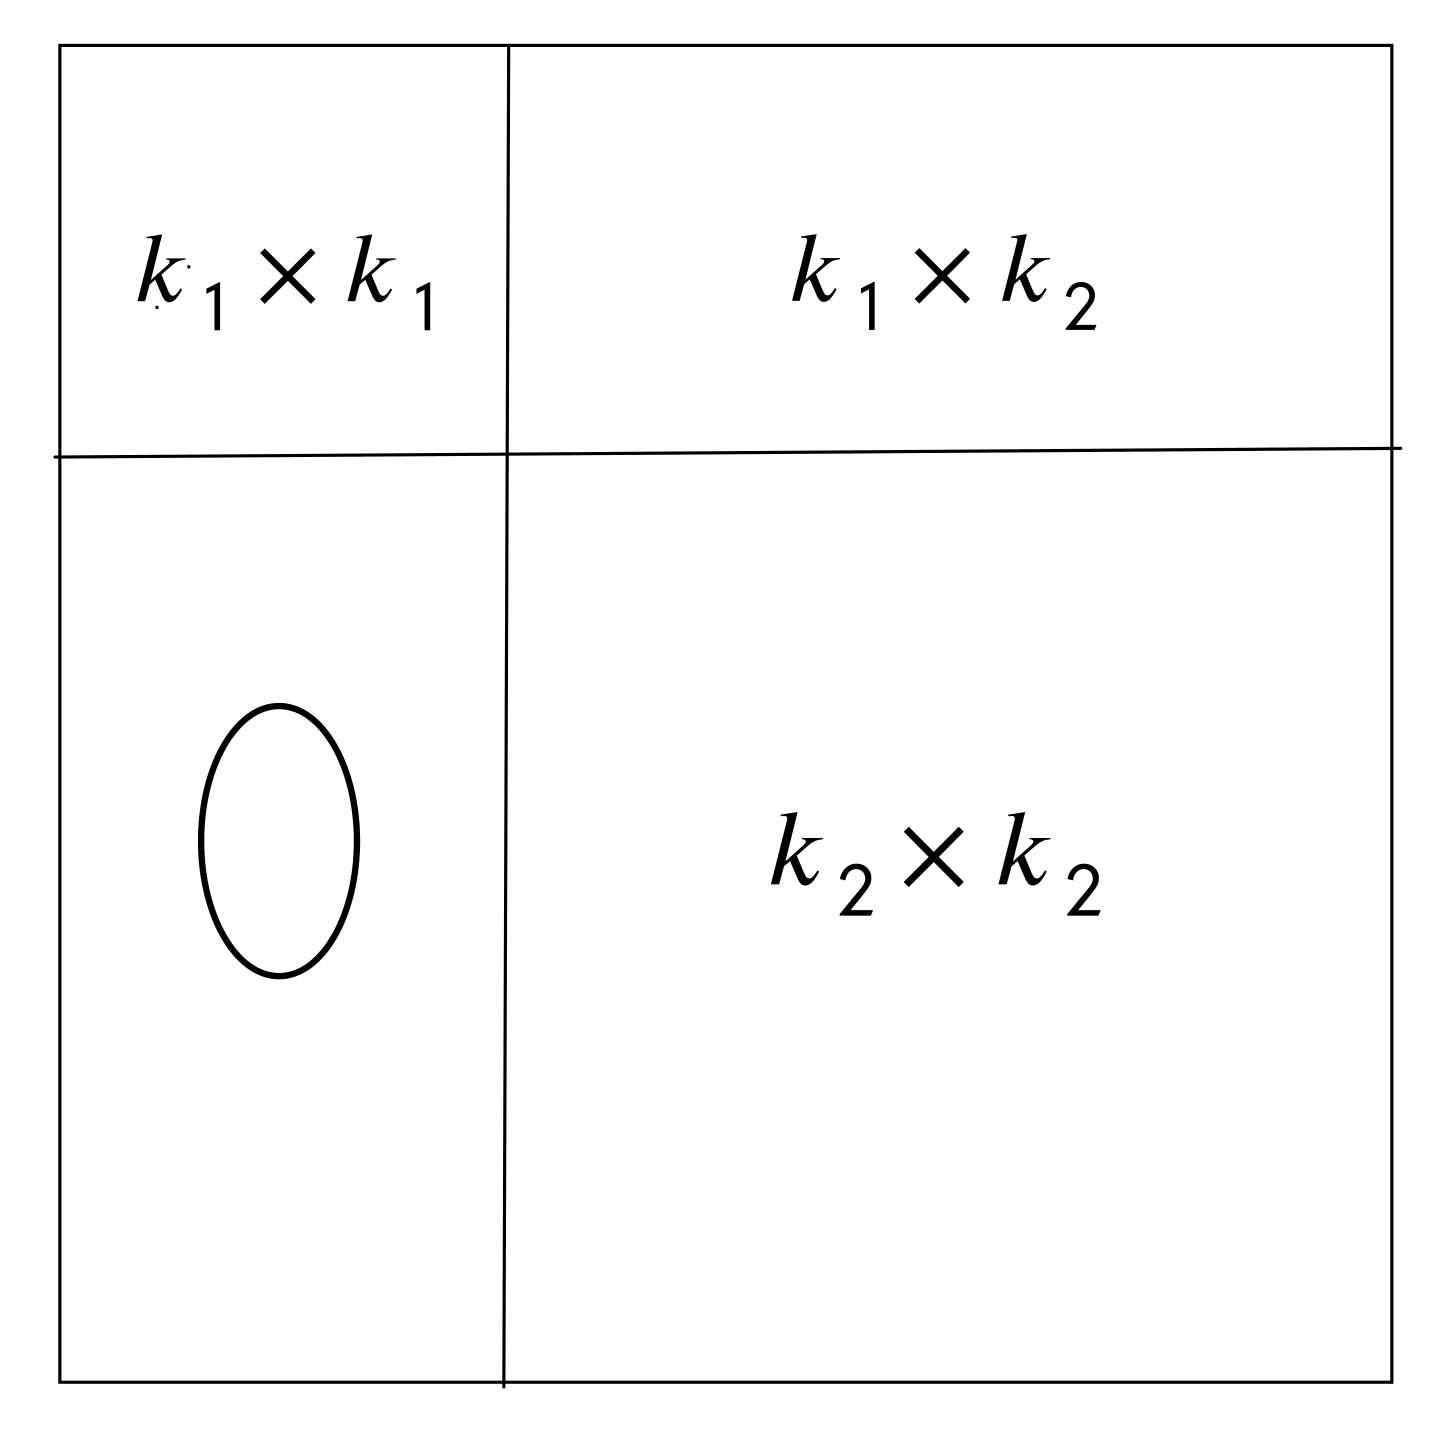
\includegraphics[scale=0.15]{1.png}
    \end{center}
    \end{figure}\\
    где $k_1 + k_2 = n, \ k_1, k_2 > 0$.
    \begin{theorem}
        У данного преобразования имеется нетривиальное инвариантное подпространство $\Leftrightarrow$ его матрица в некотором базисе \textbf{полураспавшаяся}.
    \end{theorem}
    \begin{Proof}
    Пусть линейное преобразование $\varphi$ имеет имеет инвариантное подпространство: $$\varphi(W) \subset W$$
    $\Rightarrow$ Возьмем базис подпространства $w_1, w_2, \dots, w_{k1}$ и дополним его до базиса пространства: $$w_1,w_2, \dots, w_{k1}, v_1, v_2, \dots, v_{k2}$$
    Посчитаем матрицу линейного преобразования в новом базисе:
    $$\varphi(w_1) \in W, \ \varphi(w_1)=\alpha_{11}w_1+\alpha_{21}w_2+\dots+\alpha_{k+1 \ 1}w_{k1}+0v_1+\dots+0v_{k2} \eqno(1)$$\\\\
    $\Leftarrow$ Если для линейного преобразования существует полураспавшаяся матрица, то выполнется разложение (1). А значит
    $$\begin{cases}
           \varphi(w_1) \in L(w_1, w_2, \dots, w_{k1})\\
           \varphi(w_2) \in L(w_1, w_2, \dots, w_{k1})\\
           \dotfill \\
           \varphi(w_{k1}) \in L(w_1, w_2, \dots, w_{k1})
    \end{cases}$$
    Отсюда следует, что $L$ --- инвариантно.\\\\
    Рассмотрим произвольный вектор $w$:
    $$w = \alpha_1w_1+\alpha_2w_2+\dots+\alpha_{k1}w_{k1}$$
    $$\varphi(w)=\alpha_1\varphi(w_1)+\alpha_2\varphi(w_2)+\dots+\alpha_{k1}\varphi(w_{k1})$$
    Так как $\varphi(w_i) \in L$ то и $\varphi(w) \in L$.
    \end{Proof}\\\\
    \textbf{Замечание}. Инвариантность подпространства достаточно проверять только на базисных векторах.
    \section{Характеристическая матрица и характеристический многочлен}
    Пусть $A$ --- квадратная матрица.\\
    $\bullet$ Характеристическая матрица матрицы $A$ имеет вид:
    $$xE-A$$
    $\bullet$ Характеристическим многочленом называется определитель характеристической матрицы:
    $$|xE-A|$$
    \textbf{Примеры.}
    \begin{enumerate}
        \item $A=E$ --- единичная матрица.\\
        $$(xE-E) = 
        \begin{pmatrix}
        x-1 & 0 & \dots & 0\\
        0 & x-1 & \dots & 0\\
        \vdots & \vdots & \ddots & \vdots\\
        0 & 0 & \dots & x - 1
        \end{pmatrix}, \quad
        |xE-E| = (x-1)^n$$
        \item $A = 0$ --- нулевая матрица.\\
        $$xE-0=xE= 
        \begin{pmatrix}
        x & 0 & \dots & 0\\
        0 & x & \dots & 0\\
        \vdots & \vdots & \ddots & \vdots\\
        0 & 0 & \dots & x
        \end{pmatrix}, \quad |xE-0| = x^n$$
    \end{enumerate}
    $\bullet$ \textbf{Следом} линейного преобразования называется выражение
    $$\tr \varphi = \tr A = \sum^n_{i=1}a_{ii}$$
    где $A = (a_{ij})$ --- матрица линейного преобразования $\varphi$.\\\\
    \textbf{Свойства характеристических матрицы и многочлена:}
    \begin{enumerate}
        \item \begin{itemize}
            \item \textit{Характеристическая матрица всегда невырожденная.}
            \item \textit{Характеристический многочлен всегда $\neq 0$.}
            \item \textit{Степень многочлена равна $n$ --- порядок матрицы.}
        \end{itemize}
        \item $f(x) = 
        \begin{vmatrix}
        x-a_{11} & -a_{12} & \dots & -a_{1n}\\
        -a_{21} & x-a_{22} & \dots & -a_{2n}\\
        \vdots & \vdots & \ddots & \vdots\\
        -a_{n1} & a_{n2} & \dots & x-a_{nn}
        \end{vmatrix}
        = x^n - (a_{11} + a_{22} + \dots + a_{nn})x^{n-1} + \dots$
        \item $f(0) = (-1)^n \cdot |A|$ --- свободный член.
        \item \textit{Матрица будет вырожденной $\Leftrightarrow 0 $ является корнем ее многочлена.}
        \begin{Proof}
        $f(0) = |-A| = 0$
        \end{Proof}
        \item \textit{Характеристические многочлены подобных матриц равны.}
        \begin{Proof}
        Пусть $B = S^{-1}AS$\\
        $|xE-B| = |xE - S^{-1}AS| = |S^{-1}xES - S^{-1}AS| = |S^{-1}(xE-A)S| = |S^{-1}| \cdot |xE-A| \cdot |S| = |S^{-1}| \cdot |S| \cdot |xE-A| = |S \cdot S^{-1}| \cdot |xE - A| = |E| \cdot |xE - A| = |xE - A|$
        \end{Proof}
        \item \textit{Характеристический многочлен полураспавшейся (распавшейся) матрицы равен произведению характеристических многочленов ее диагональных блоков.}
        $$\begin{pmatrix}
        A_1 & C\\
        0 & A_2
        \end{pmatrix}, \quad 
        \begin{vmatrix}
        xE_{n1}-A_1 & -C\\
        0 & xE_{n2}-A_2
        \end{vmatrix} = |xE_{n1}-A_1|\cdot|xE_{n2}-A_2|$$
    \end{enumerate}
    \section{Собственные векторы и собственные значения линейного преобразования}
    Пусть $\varphi$ --- линейное преобразование пространства $V_n$.\\
    $\bullet$ $\vec x \neq 0$ --- \textbf{собственный вектор} линейного преобразования $\varphi$, отвечающий собственному значению $\lambda$:
    $$\varphi(x) = \lambda x$$
    \textbf{Примеры}
    \begin{enumerate}
        \item $\varphi(v) = v$ --- тождественное преобразование.\\
        Все векторы собственные, отвечают значению 1.
        $$\varphi(v) = 1 \cdot v$$
        \item $\varphi(v) = \vec 0$ --- нулевое преобразование.\\
        Все векторы собственные, отвечают значению 0.
        $$\varphi(v) = \vec 0 = 0 \cdot v$$
        \item Проектирование\\
        Векторы прямой: $\varphi(\vec a) = 1 \cdot \vec a$ --- отвечают значению 1.\\
        Векторы перпендикулярной плоскости: $\varphi(\vec a) = \vec 0 = 0 \cdot \vec a$ --- отвечают значению 0.
    \end{enumerate}
    $$X \stackrel{\varphi}{\rightarrow} AX$$
    $$AX = \lambda X$$
    $$AX = \lambda EA$$
    $$(A - \lambda E)X = 0 \sim (A-\lambda E|0)$$
    То есть решения ОСЛУ образуют векторное пространство.
    $$\varphi(x)=\lambda x \sim (\varphi - \lambda e)x = \vec 0$$
    Образует инвариантное подпространство.
    \begin{theorem}
        Собственные значения линейного преобразования --- это корни характеристического многочлена (характеристические числа, принадлежащие основному полю).
    \end{theorem}
    \begin{Proof}
    По определению $\varphi(x)=\lambda x$. Запишем условие существования собственного вектора в виде:
    $$(\varphi-\lambda E)x = \vec 0$$
    Так как $\vec x \neq 0$ по определению, то преобразование $\varphi - \lambda e$ должно быть вырожденным:
    $$\det (\varphi - \lambda e) = 0 \eqno (1)$$
    Пусть в каком-нибудь базисе преобразование $\varphi$ имеет матрицу $A$, тогда преобразование $\varphi - \lambda e$ будет иметь матрицу $A - \lambda E$.\\
    Тогда условие (1) можно записать в следующем виде:
    $$\det (A - \lambda E) = 
    \begin{vmatrix}
    a_{11}-\lambda & a_{12} & \dots & a_{1n}\\
    a_{21} & a_{22} - \lambda & \dots & a_{2n}\\
    \vdots & \vdots & \ddots & \vdots\\
    a_{n1} & a_{n2} & \dots & a_{nn} - \lambda
    \end{vmatrix} = 0$$
    А $\det(A - \lambda E)$ --- характеристический многочлен, корнями которого являются собственные значения $\lambda$.
    \end{Proof}
    Собственные векторы, отвечающие найденным собственным значениям, и нулевой вектор образуют инвариантное подпространство $\ker (\varphi - \lambda e)$, и их можно найти, решая ОСЛУ $(A - \lambda E|0)$ и отбрасывая 0.
    \begin{theorem}
        Собственные векторы, отвечающие попарно различным собственным значениям, линейно независимы.
    \end{theorem}
    \begin{Proof}
    Пусть $\lambda_1, \lambda_2, \dots, \lambda_k, \ \lambda_i \neq \lambda_j, \ i \neq j$ --- некоторые собственные значения.\\
    $\varphi(x_i) = \lambda_i x_i, \ i = 1, 2, \dots, k$ --- собственные векторы.
    Докажем теорему методом от противного.\\
    Предположим, что векторы линейно зависимы. Следовательно, один вектор линейно выражается через все остальные, которые будут линейно независимы:
    $$x_k = \alpha_1x_1+\alpha_2x_2+\dots+\alpha_{k-1}x_{k-1} \eqno(2)$$
    где $x_1, x_2, \dots, x_{k-1}$ --- линейно независимы.
    Подействуем на обе части уравнения (2) линейным преобразованием $\varphi$:
    $$\lambda_kx_k = \alpha_1\lambda_1x_1+\alpha_2\lambda_2x_2+\dots+\alpha_{k-1}\lambda_{k-1}x_{k-1} \eqno(3)$$
    Умножим обе части уравнения (2) на $\lambda_k$:
    $$\lambda_kx_k = \alpha_1\lambda_kx_1+\alpha_2\lambda_kx_2+\dots+\alpha_{k-1}\lambda_kx_{k-1} \eqno(4)$$
    Вычтем из уравнения (3) уравнение (4):
    $$\alpha_1(\lambda_1-\lambda_k)x_1+\alpha_2(\lambda_2-\lambda_k)x_2+\dots+\alpha_{k-1}(\lambda_{k-1}-\lambda_k)x_{k-1} = \vec 0$$
    Так как векторы $x_i$ линейно независимы, то $\alpha_i(\lambda_i-\lambda_k) = 0, \ i = 1, 2, \dots, k-1$.\\
    Так как вектор $x_k \neq 0$, то $\alpha_i \neq 0$ одновременно. Положим, что $\alpha_1 \neq 0$.\\
    Так как $\alpha_1 \neq 0, \ \lambda_k \neq \lambda_i \Rightarrow \alpha_i(\lambda_1-\lambda_k) \neq 0$.\\
    Полученное противоречие доказывает наше утверждение.
    \end{Proof}
    \begin{theorem}
        Если у преобразования $\varphi$ пространства $V_n$ имеется $n$ попарно различных собственных значений, то для него существует базис, состоящий из собственных векторов, отвечающих этим значениям, и его матрица в этом базисе будет диагональной.
    \end{theorem}
    \begin{Proof}
    Пусть $\lambda_1, \lambda_2, \dots, \lambda_n, \ \lambda_i \neq \lambda_j, \ i \neq j$ --- собственные значения.\\
    $v_1, v_2, \dots, v_n$ --- векторы, отвечающие данным значениям.\\
    Разложим эти векторы:
    $$\begin{cases}
           \varphi(v_1)=\lambda_1v_1+0v_2+\dots+0v_n\\
           \varphi(v_2)=0v_1+\lambda_2v_2+\dots+0v_n\\
           \dotfill\\
           \varphi(v_n)=0v_1+0v_2+\dots+\lambda_nv_n\\
    \end{cases}$$
    Тогда матрица преобразования имеет вид:
    $$\begin{pmatrix}
    \lambda_1 & 0 & \dots & 0\\
    0 & \lambda_2 & \dots & 0\\
    \vdots & \vdots & \ddots & \vdots\\
    0 & 0 & \dots & \lambda_n
    \end{pmatrix}$$
    \end{Proof}\\
    \textbf{Следствие.} \textit{Если у квадратной матрицы имеется $n$ попарно различных характеристических чисел, то эта матрица подобна диагональной.}
    \section{Основные свойства делимости в кольце целых чисел}
    $\N = \{ 1, 2, \dots \}$\\
    $\Z = \{ 0, \pm 1, \pm 2, \dots \}$\\\\
    $\bullet$ Говорят, что $a$ делит $b \ (a | b)$, когда $a \neq 0$ и $\exists q: \ b=aq$.\\\\
    \textbf{Свойства делимости:}
    \begin{enumerate}
        \item $b|a, \ b|c \Rightarrow b|a\pm c$
        \begin{Proof}
        $a=bq_1$\\
        $c=bq_2$\\
        $a \pm c = b(q_1 \pm q_2)$
        \end{Proof}
        \item $b | a \Rightarrow b |ac$
        \begin{Proof}
        $a=bq_1$\\
        $ac=bq_1c$
        \end{Proof}
        \item $a|b, \ b|a \Leftrightarrow a= \pm b$
        \begin{Proof}
        $b=aq_1$\\
        $a=bq_2$\\
        $b=bq_2q_1$\\
        $1=q_1q_2 \Leftrightarrow \left[ 
        \begin{gathered}
            q_2=q_1=-1\\
            q_2=q_1=1
        \end{gathered} \right.$
        \end{Proof}
        \item $b |a \Rightarrow (a,b)=b$
    \end{enumerate}
    \begin{theorem}
        Всякое число $a$ представимо единственным образом через положительное $b$ в виде
        $$a=bq+r, \quad 0 \leq r < b$$
    \end{theorem}
    \begin{Proof}
    Возьмем наибольшее $q$ с условием, что $bq \leq a$.\\
    Тогда $r=a-bq \ \Rightarrow r$ удовлетворяет условию  $0 \leq r < b$.\\
    Покажем однозначность:\\
    $$a=bq+r$$
    $$a=bq_1+r_1$$
    Вычтем из одного равенства другое:
    $$b(q-q_1)=r_1-r$$
    Очевидно, что $r_1-r < b$. Пусть тогда $r_1>r$. Тогда $q-q_1>0 \ \Rightarrow$ равенство невозможно $\Rightarrow \ r=r_1 \Rightarrow \ r_1-r=0$.\\
    А так как $b \neq 0$, то $q-q_1=0 \ \Rightarrow q=q_1$.
    \end{Proof}
    \subsection{НОД}
    $\bullet$ \textbf{НОД} --- наибольший общий делитель 2 чисел, обозначается $(a, b)$.\\\\
    \textbf{Свойства НОДа:}
    \begin{enumerate}
        \item Для $(0, 0)$ НОД не существует.
        \item $(a, 0) = a, \ a \neq 0$.
        \item Знак не влияет на делимость.
        \item $a=bq+r \ \Rightarrow (a,b)=(b,r)$
        \begin{Proof}
        Если $d|a$ и $d|b \ \Rightarrow \ d|r$.\\
        Если $d|r$ и $d|b \ \Rightarrow \ d|a$.
        \end{Proof}
    \end{enumerate}
    \subsection{Алгоритм Евклида}
    \begin{enumerate}
        \item \textit{Большее из чисел поделить с остатком на меньшее:}
        $$a=bq_1+r_1$$
        \item \textit{Делитель делим с остатком на остаток $r_1$:}
        $$b=r_1q_2+r_2$$
        \item \textit{Продолжаем до тех пор, пока не получим первый нулевой остаток. Последний, отличный от 0 остаток, будет НОДом.}
        $$r_1=r_2q_3+r_3$$
        $$r_{n-1}=r_nq_{n+1}+r_{n+1}$$
        $$r_n=r_{n+1}q_{n+2}$$
        $$(a,b)=r_{n+1}$$
        \begin{Proof}
        $$(a,b)=(b,r_1)=(r_1,r_2)=\dots=r_{n+1}$$
        \end{Proof}
    \end{enumerate}
    \subsection{Расширенный алгоритм Евклида}
    Под расширенным алгоритмом Евклида, или линейным разложением НОДа, понимается представление НОДа в виде:
    $$d=au+bv$$
    \section{Взаимно простые числа}
    $\bullet$ Числа $a, b$ называются \textbf{взаимно простыми}, если их НОД равен 1, то есть
    $$(a,b)=1$$
    \begin{theorem}
        \textbf{Критерий взаимной простоты}
        $$(a,b)=1 \Leftrightarrow \exists u, v \ au+bv=1$$.
    \end{theorem}
    \begin{Proof}
    $\Rightarrow$ По расширенному алгоритму Евклида $d=au+bv$.\\
    Так как $(a,b)=1$, то $1=au+bv$.\\\\
    $\Leftarrow$ Всякий делитель $a$ и $b$ будет делителем 1.
    \end{Proof}\\\\
    \textbf{Свойства взаимно простых чисел}
    \begin{enumerate}
        \item $a|bc$, $(a,b)=1 \Rightarrow a|c$ 
        \begin{Proof}
        $$au+bv=1$$
        Умножим обе части равенства на $c$.
        $$acu+bcv=c$$
        Так как $a|acu$, $a|bcv$ ($a|bc$ по условию), то $a|c$.
        \end{Proof}
        \item $a,b|c, \ (a,b)=1 \ \Rightarrow \ ab|c$
        \begin{Proof}
        $$au+bv=1$$
        Умножим обе части равенства на $c$.
        $$acu+bcv=c$$
        Так как $ab|acu$, $ab|bcv$, то $ab|c$.
        \end{Proof}
        \item $(a,c)=(b,c)=1 \Rightarrow (ab,c)=1$
    \end{enumerate}
    \section{НОК}
    Под наименьшим общим кратным понимается наименьшее число, которое делят и $a$, и $b$.
    \begin{theorem}
        $$a|M, \ b|M \ \Rightarrow [a,b]|M$$
    \end{theorem}
    \begin{Proof}
    $$M=[a,b]q+r$$
    $$a|M, \ a|[a,b] \Rightarrow a|r$$
    $$b|M, \ b|[a,b] \Rightarrow b|r$$
    $$a,b|r, \ r<[a,b] \Rightarrow r=0$$
    \end{Proof}
    \begin{theorem}
        $$ab=(a,b)[a,b]$$
    \end{theorem}
    $\bullet$ $[ak, bk] = [a,b]k$\\\\
    НОД и НОК можно вычислять последовательно:
    $$(a,b,c)=((a,b),c)$$
    $$[a,b,c,d]=[[a,b,c],d]=[[a,b],c],d]$$
    \section{Простые числа}
    Число $p>1, \ p \in \N$ называется простым, если $1|p$ и $p|p$, других делителей нет.\\\\
    $\bullet$ Либо $(p,a)=1$ --- $p$ взаимно простое с $a$, либо $p|a$.
    \begin{theorem}
        Простых чисел бесконечно много.
    \end{theorem}
    \begin{Proof}
    Если число простых чисел конечно, то их можно перечислить и перемножить:
    $$2\cdot3\cdot \ \dots \ \cdot p$$
    Добавим 1:
    $$2\cdot3\cdot \ \dots \ \cdot p +1$$
    Полученное число не может быть простым, так как простые числа мы перечислили в произведении. Значит оно составное.\\
    Если это число составное, то оно должно раскладываться на простые делители, при этом $q \neq 2,3,\dots \ \Rightarrow$ число должно иметь другие простые числа, которые его делят, или само быть простым.\\
    Так как оба условия невозможны, то получаем противоречие.
    \end{Proof}\\
    \begin{theorem}
        Любое число представимо в виде степеней попарно простых чисел:
        $$m=p_1^{k_1}\cdot p_2^{k_2}\cdot \ \dots \ \cdot p_r^{k_r}$$
    \end{theorem}
    \begin{Proof}
    \textbf{Возможность}\\
    $m=m_1 \cdot p_1$, где $p_1$ --- наименьший простой делитель.\\
    Если $m_1>1$, то $m=m_2 \cdot p_1 \cdot p_2$ и т.д., пока $p_i \neq 1$.
    В конечном итоге получим разложение:
    $$m=p_1\cdot p_2\cdot p_3\cdot \ \dots \ \cdot p_i$$
    где $p_i = 1$.\\
    С учетом кратности простых чисел в полученном разложении, его можно переписать в виде:
    $$m=p_1^{k_1}\cdot p_2^{k_2}\cdot \ \dots \ \cdot p_r^{k_r}$$
    \textbf{Единственность}\\
    Пусть $m=p_1\cdot p_2 \cdot \ \dots \ \cdot p_l$ и $m=q_1 \cdot q_2 \cdot \ \dots \ \cdot q_s$.\\
    Следовательно $p_1\cdot p_2 \cdot \ \dots \ \cdot p_l=q_1 \cdot q_2 \cdot \ \dots \ \cdot q_s$.\\
    Так как левая часть делится на $p_1$, то и правая часть тоже. Значит среди множителей правой части есть хотя бы один, который делится на $p_1$.\\
    А так как все они простые, то какой-то из множителей равен $p_1$ (пусть это $q_1$), значит на него можно сократить.\\
    Продолжая алгоритм до конца, приходим к выводу, что все множители обеих частей попарно равны.
    \end{Proof}
    \section{Сравнения}
    Возьмем $m \in \N, \ m>1$.\\\\
    $a$ и $b$ \textbf{сравнимы по модулю $m$}, если у $a$ и $b$ одинаковый остаток при делении на $m$.\\
    $\bullet$ $a \equiv b \ (\mod m), \ m|a-b$\\\\
    \textbf{Пример}\\
    $10 \equiv 12 \ (\mod 2)$,
    так как $10 \mod 2 = 12 \mod 2 = 0$.\\\\
    \textbf{Свойства сравнений}
    \begin{enumerate}
        \item $a \equiv a \ (\mod m)$ --- \textit{рефлексивность.}
        \item $a \equiv b \ (\mod m) \Rightarrow b \equiv a \ (\mod m)$ --- \textit{симметричность.}
        \item $a \equiv b \ (\mod m), \ b \equiv c \ (\mod m) \Rightarrow a \equiv c \ (\mod m)$ --- \textit{транзитивность.}
        \item  $a \equiv b \ (\mod m) \Rightarrow a+c \equiv b+c \ (\mod m)$\\\\
        $m|(a+c)-(b+c)=a-b$
        \item \textit{Сравнения по одному и тому же модулю можно почленно складывать}\\
        $$a \equiv b \ (\mod m)$$
        $$a^\prime \equiv b^\prime \ (\mod m)$$
        $$a+a^\prime \equiv b+b^\prime \ (\mod m)$$
        $$m|(a+a^\prime-(b+b^\prime))=(a-b)+(a^\prime+b^\prime)$$
        \item \textit{Сравнения по одному и тому же модулю можно почленно умножать}
        $$a\cdot a^\prime \equiv b \cdot b^\prime \ (\mod m)$$
        $$a=mq_1+r_1$$
        $$a^\prime=mq_2+r_2$$
        $$a\cdot a^\prime = mQ_1+r_1r_2$$
        $$b=mq_3+r_1$$
        $$b^\prime=mq_4+r_2$$
        $$b\cdot b^\prime = mQ_2+r_1r_2$$
        $$m|aa^\prime-bb^\prime=m(Q_1-Q_2)$$
        \item \textit{Обе части сравнения можно умножить на одно и то же число}
        $$a \equiv b \ (\mod m)$$
        $$ak \equiv bk \ (\mod m)$$
        $$m|k(a-b)$$
        \item \textit{Обе части сравнения и модуль можно умножать на одно и то же число}
        $$a \equiv b \ (\mod m)$$
        $$ak \equiv bk \ (\mod mk)$$
        $$mk|k(a-b)$$
        \item \textit{Обе части сравнения и модуль можно сокращать на одно и то же число}
        $$ak \equiv bk \ (\mod mk) \Rightarrow a \equiv b \ (\mod m)$$
        $$\dfrac{(a-b)k}{mk}=\dfrac{a-b}{m}$$
        \item \textit{Обе части сравнения можно сокращать на число, взаимно простое с модулем.}
        $$ak \equiv bk \ (\mod m) \Rightarrow a \equiv b \ (\mod m), \ (k,m)=1$$
        $$m|k(a-b)$$
        \item $a \equiv b \ (\mod m) \Rightarrow (a,m)=(b,m)$\\
        $a=b+km$
    \end{enumerate}
    \section{Классы вычетов}
    $\bullet$ В класс вычетов входят все числа с данным остатком.\\
    $\bullet$ Класс вычетов определяет бинарное отношение эквивалентности.\\\\
    \textbf{Пример}\\
    $$m = 3: \ 3\Z, \ 3\Z+1, \ 3\Z+2$$
    $\bullet$ \textbf{Вычет} --- любой элемент класса.\\
    $\bullet$ $\bar{a}$ --- класс, в который входят элементы с таким же остатком, как у $a$.\\\\
    \textbf{Пример}
    $$\bar{1}=\{2k+1\}, \ m=2$$
    $\bullet$ $\bar{a} = \bar{b}$ --- классы совпадают $\Leftrightarrow \ a \equiv b \ (\mod m)$\\
    $\bullet$ $\bar{a} = \bar{b}$ либо $\bar{a} \cap \bar{b} = \varnothing$\\
    $\bullet$ \textbf{Полной системой вычетов} называется система представителей всех классов вычетов.
    \begin{theorem}
        Пусть $(a,m)=1$, $x$ пробегает полную систему вычетов $\Rightarrow \ ax+b$ пробегает полную систему вычетов.
    \end{theorem}
    \begin{Proof}
    Рассмотрим вычеты $x_1$ и $x_2$, которые относятся к разным классам (1).\\
    Предположим, что $ax_1+b \equiv ax_2+b \ (\mod m)$.\\
    Тогда по свойству \textbf{4} мы можем отнять число $b$. А так как по условию $(a,m)=1$, то по свойству \textbf{10} можно сократить на число $a$.\\
    Таким образом получим $$x_1 \equiv x_2 \ (\mod m)$$
    что противоречит условию (1).
    \end{Proof}\\
    $\bullet$ Полная система вычетов: $m: 0,1,2, \dots, m-1$.\\
    $\bullet$ Приведенная система вычетов: взаимно простые с модулем числа.\\
    $\bullet$ Если один представитель класса взаимно простой с модулем, то все элементы класса взаимно простые с модулем.
    \begin{theorem}
        Пусть $(a,m)=1$. Тогда $x$ и $ax$ одноименно пробегают приведенную систему вычетов или нет.
    \end{theorem}
    \begin{Proof}
    $ax_1 \equiv ax_2 \ (\mod m) \Leftrightarrow x_1 \equiv x_2 \ (\mod m)$
    \end{Proof}
    \section{Функция Эйлера}
    Определяется для любого натурального $m$.\\
    $\bullet$ $\varphi(m)$ --- число классов вычетов, взаимно простых с модулем.\\\\
    \textbf{Пример}\\
    $\varphi(1)=1$\\
    $\varphi(2)=1$ --- классы вычетов $(0,1)$, но $0$ не взаимно простой с $2$.\\
    $\varphi(3) = 2$  --- классы вычетов $(0,1,2)$, но $0$ не взаимно простой с $3$.\\
    $\varphi(4) = 2$\\
    $\varphi(5) = 4$
    \begin{theorem}
        $\varphi(p)=p-1$, где $p$ --- простое число.
    \end{theorem}
    \begin{Proof}
    Полная система вычетов для $p$: $0,1,2,\dots,p-1$.\\
    Так как $p$ --- простое число, то все вычеты с ним взаимно простые.
    \end{Proof}
    \begin{theorem}
        $\varphi(p^n)=p^n-p^{n-1}$
    \end{theorem}
    \begin{Proof}
    $$1,2,\dots,p,\dots,2p,\dots,p^n-1,p^n$$
    В этом ряду каждое $p$-ое число делится на $p$, остальные взаимно простые, следовательно
    $$p^n-\dfrac{p_n}{p}=p^n-p^{n-1}$$
    \end{Proof}
    \begin{theorem}
        $(a,b)=1 \Rightarrow \varphi(ab)=\varphi(a)\varphi(b)$
    \end{theorem}
    \begin{Proof}
    Запишем матрицу
    $$\begin{pmatrix}
    1 & 2 & 3 & \dots & a\\
    a+1 & a+2 & a+3 & \dots & 2a\\
    \vdots & \vdots & \vdots & \ddots & \vdots\\
    (b-1)a+1 & (b-1)a+2 & (b-1)a+3 & \dots & ab
    \end{pmatrix}$$
    Найдем числа такие, что $(x,ab)=1$.
    $$(x,ab)=1 \Leftrightarrow (x,a)=(x,b)=1$$
    Вначале ищем $x$ взаимно простые с $a$. Эти числа могут быть только в столбцах с номерами, взаимно простыми с $a$. А таких столбцов $\varphi(a)$.\\
    Более того, все числа таких столбцов взаимно простые с $a$ и этот столбец --- полная система вычетов по модулю $b$.\\
    Значит чисел взаимно простых с $b$ --- $\varphi(b)$.\\
    Тогда $\varphi(ab)=\varphi(a)\varphi(b)$.
    \end{Proof}
    \begin{theorem}
        \textbf{Эйлера}\\
        $(a,m)=1 \Rightarrow a^{\varphi(m)} \equiv 1 \ (\mod m)$
    \end{theorem}
    \begin{Proof}
    Возьмем такое $a$, что $(a,m)=1$.\\
    Пусть $l=\varphi(m)$.\\
    И возьмем приведенную систему вычетов $\varepsilon_1,\varepsilon_2,\dots,\varepsilon_l$.\\
    Рассмотрим сравнение $$(a\varepsilon_1)\cdot(a\varepsilon_2)\cdot \ \dots \ (a\varepsilon_l) \equiv \varepsilon_1\cdot\varepsilon_2\cdot \ \dots \ \varepsilon_l \ (\mod m)$$ 
    Так как мы взяли приведенную систему вычетов, то $\varepsilon_i$ взаимно простое с $m$, значит мы можем сократить на все $\varepsilon$ обе части.\\
    В конце получим
    $$a^{\varphi(m)} \equiv 1 \ (\mod m)$$
    \end{Proof}
    \begin{theorem}
        \textbf{Ферма}\\
        $(a,p)=1 \Rightarrow a^{p-1} \equiv 1 \ (\mod m)$
    \end{theorem}
    \begin{Proof}
    Доказательство следует из предыдущей теоремы.\\
    Используем лемму о том, что $\varphi(p)=p-1$ и подставим это значение в $a^{\varphi(m)} \equiv 1 \ (\mod m)$.\\
    Получаем
    $$a^{p-1} \equiv 1 \ (\mod m)$$
    \end{Proof}
    \section{RSA-криптосистема}
    $\bullet$ С помощью теоремы Эйлера появилась первая система цифровой подписи и первая криптосистема с открытым ключом.\\
    Рассмотрим факторизацию числа $N$:
    $$N=pq$$
    Найдем значение функции Эйлера:
    $$\varphi(N)=(p-1)(q-1)$$
    Далее подбираются числа $e$ и $d$ такие, что
    $$ed \equiv 1 \ (\mod c), \ c=\varphi(N)$$
    $e$ --- \textbf{открытый} ключ.\\
    $d$ --- \textbf{закрытый} ключ.\\\\
    \textbf{Шифрование}\\
    Берем число $x$ такое, что $(x,N)=1$.
    $$x \rightarrow x^e \mod N$$
    \textbf{Дешифрование}
    $$x^e = (x^e)^d \mod N$$
    \begin{Proof}
    $x^{ed} = x^{1+ke} = (x^e)^k\cdot x \equiv x \ (\mod N)$\\
    Так как $(x,N)=1$, можно сократить на $x$:
    $$(x^e)^k \equiv 1 \ (\mod N)$$
    \end{Proof}
    \section{Сравнения первой степени}
    $$ax \equiv b \ (\mod m)$$
    \begin{theorem}
        Сравнение разрешимо $\Leftrightarrow \ d|b$. В случае разрешимости оно имеет единственное решение по модулю $m^\prime$ и $d$ решений по модулю $m$: $$x \equiv x_0, x_0 + \dfrac{m}{d}, x_0+2\dfrac{m}{d}, \dots, (d-1)\dfrac{m}{d}$$
    \end{theorem}
    \begin{Proof}
        $(a,m) = d | b$ --- необходимое условие разрешимости.
        $$\dfrac{ax-b}{m} \in \Z$$
        $d | ax$  и $d | m$ (так как $d = (a, m) )\ \Rightarrow d | b$.\\
        Поделим обе части сравнения и модуль на $d$.
        $$\dfrac{a}{d}x \equiv \dfrac{b}{d} \ (\mod \dfrac{m}{d})$$
        Обозначим как $$a^\prime x \equiv b^\prime \ (\mod m^\prime), \ (a^\prime, m^\prime)=1$$
        И тогда это сравнение имеет единственное решение по модулю $m^\prime$ по 2 лемме о пробегании.\\
        Таким образом условие $(a,m) = d | b$ является и достаточным.
    \end{Proof}\\\\
    \textbf{Способы решения}
    \begin{enumerate}
        \item \textit{Подбор (при маленьком модуле)}
        $$5x \equiv 1 \ (\mod 7)$$
        Проверяем полную систему вычетов по модулю $7$:
        $$0, 1, 2, 3, 4, 5, 6$$
        $$x \equiv 3 \ (\mod 7)$$
        \item \textit{Способ Эйлера}\\
        Проверяем условие разрешимости по теореме.\\
        Если решения есть, то домножим обе части сравнения на $a^{\varphi(m)-1}$:
        $$a^{\varphi(m)-1}ax \equiv ba^{\varphi(m)-1} \ (\mod m)$$
        По теореме Эйлера $$a^{\varphi(m)} \equiv 1 \ (\mod m) \Rightarrow \ x \equiv ba^{\varphi(m)-1} \ (\mod m)$$
        \item \textit{Расширенный алгоритм Евклида}\\
        Нужно найти такие $u$ и $v$, что 
        $$au+mv=1$$
        Домножим обе части сравнения на $u$:
        $$aux \equiv bu \ (\mod m)$$
        $$(1-mv)x \equiv bu \ (\mod m)$$
        $$mv \equiv 0 \ (\mod m) \Rightarrow \ x \equiv bu \ (\mod m)$$
    \end{enumerate}
\section{Системы сравнений}
    $\begin{cases}
           a_1x \equiv b_1 \ (\mod m_1)\\
           a_2x \equiv b_2 \ (\mod m_2)\\
           \dotfill\\
           a_sx \equiv b_s \ (\mod m_s)
    \end{cases}$ сводится к \
    $\begin{cases}
           x \equiv c_1 \ (\mod m_1)\\
           x \equiv c_2 \ (\mod m_2)\\
           \dotfill\\
           x \equiv c_s \ (\mod m_s)\\
    \end{cases}$\\\\
    \textbf{Способ 1}\\
    Выражаем $x$ из первого cравнения
    $$x = c_1 + m_1t\eqno(1)$$
    и подставляем во второе.\\
    Находим оттуда $t$ и подставляем в уравнение (1):
    $$m_1t \equiv (c_2-c_1) \ (\mod m_2), \ (m_1, m_2) | c_2-c_1$$
    $$t=t_0+\dfrac{m_2}{(m_1, m_2)}k, \ k \in \Z$$
    Подставляя $t$ в уравнение (1), получаем:
    $$x = c_1 + m_1t_0 + \dfrac{m_1m_2}{(m_1, m_2)}k \Rightarrow \ x = x_0+[m_1, m_2]k$$
    где $x_0 = c_1 + m_1t$.\\
    Тогда вместо первых двух сравнений в систему запишем
    $$x \equiv x_0 \ (\mod [m_1, m_2])$$
    Этот алгоритм либо установит неразрешимость системы, либо найдет одно решение по модулю $[m_1, m_2, \dots, m_s]$.\\\\
    \textbf{CRT (Китайская теорема об остатках)}\\
    Предназначена для решения систем вида:
    $\begin{cases}
           x \equiv c_1 \ (\mod m_1)\\
           x \equiv c_2 \ (\mod m_2)\\
           \dotfill\\
           x \equiv c_s \ (\mod m_s)
    \end{cases} \ (m_i, m_j) = 1, \ i \neq j$\\
    Домножим каждое сравнение на модули других сравнений (имеем право, так как модули попарно взаимно простые):
    $$\begin{cases}
           x_1m_2m_3\dots m_s \equiv 1 \ (\mod m_1)\\
           x_2m_21m_3\dots m_s \equiv 1 \ (\mod m_2)\\
           \dotfill\\
           x_sm_1m_2\dots m_{s-1} \equiv 1 \ (\mod m_s)
    \end{cases}$$
    Все они разрешимы по критерию разрешимости: $(a, m) = 1 | 1$.\\
    Составляем решение:
    $$X = c_1x_1m_2m_3\dots m_s + c_2x_2m_1m_3\dots m_s + \dots + c_sx_sm_1m_2\dots m_{s-1}$$
    Так как все модули попарно взаимно простые, то их НОК = $m_1m_2\dots m_s$.\\
    \begin{theorem}
        Система сравнений с попарно взаимно простыми модулями разрешима и имеет единственное решение
        $$x \equiv c \ (\mod m_1m_2 \dots m_s)$$
    \end{theorem}
\section{Показатели}
$$a^{\varphi(m)} \equiv 1 \ (\mod m), \ (a, m) = 1$$
$\bullet$ $a \sim \delta$, если $a^\delta \equiv 1 \ (\mod m), \delta \in \N, \delta - min$.\\\\
\textbf{Свойства показателя}
\begin{enumerate}
    \item $a^k \equiv 1 \ (\mod m) \Rightarrow \delta | k$
    \begin{Proof}
        $$k = \delta q + r, \ 0 \leq r \leq \delta$$
        $$a^k = a^{\delta q} \cdot a^r$$
        $$a^{\delta q} \equiv 1 \ (\mod m) \Rightarrow a^k \equiv a^r \equiv 1 (\mod m)$$
        Так как $0 \leq r \leq \delta$ и $a^r \equiv 1 \ (\mod m)$, то $r = 0$. 
    \end{Proof}
    \item $a^{\varphi(m)} \equiv 1 \ (\mod m) \Rightarrow \delta | \varphi(m)$
    \item $a^0 = 1, a^1, \dots, a^{\delta -1 }$ --- в этом ряду все числа попарно не сравнимы по модулю $m$.
    \begin{Proof}
        $$a^i \equiv a^j \ (\mod m), \ i < j$$
        где $i > 0, \ j \leq \delta -1$.\\
        Сократим обе части сравнения на $a^j$:
        $$a^{i-j} \equiv 1 \ (\mod m), \ i - j < \delta$$
        Однако $\delta - min \ \Rightarrow$ противоречие.
    \end{Proof}
    \item $a \sim \delta_1, \ b \sim \delta_2, \ (\delta_1, \delta_2) = 1 \Rightarrow \ ab \sim \delta_1\delta_2$
    \begin{Proof}
        Пусть $ab \sim \delta, \ \delta \leq \delta_1\delta_2$, так как $(ab)^{\delta_1\delta_2} \equiv 1 \ (\mod m)$.\\
        $1 \equiv ((ab)^{\delta_1})^{\delta_2} \equiv a^\delta b^{\delta_1\delta_2} \equiv  a^\delta \ (\mod m) \Rightarrow \ \delta_1 | \delta, \ \delta_2 | \delta \Rightarrow \delta_1\delta_2 | \delta \ ((\delta_1, \delta_2)=1) \Rightarrow \delta_1\delta_2=\delta$.
    \end{Proof}
    \item $a \sim \delta \Rightarrow \ a^k \sim \dfrac{\delta}{(k, \delta)}$
    \begin{Proof}
        $(a^k)^l$\\
        Так как $a^m \equiv 1 \Rightarrow \delta | m$, то необходимо найти при каком минимальном значении $l$ дробь $\dfrac{kl}{\delta}$ целая.
        $$\dfrac{kl}{\delta} = \dfrac{k/(\delta, k)l}{\delta/(\delta, k)} \Rightarrow l = \dfrac{\delta}{(\delta, k)}$$
    \end{Proof}
\end{enumerate}
\section{Первообразные корни}
$$a^\delta \equiv 1 \ (\mod m)$$
$\bullet$ Первообразный корень по модулю $m$ --- число $g$ такое, что $g \sim \delta = \varphi(m)$.
\begin{theorem}
    Первообразный корень может быть только при $m=2, 4, p, p^k, 2p^k$.
\end{theorem}
\begin{Proof}
    Рассмотрим $2^k$.\\
    Пусть $k=1$. Тогда $2^k = 2, \ \varphi(2) = 1$. Первообразным корнем по модулю $2$ будет $1 \equiv -1 \ (\mod 2)$.\\
    Пусть $k=2$. Тогда $2^k = 4, \ \varphi(2) = 2$. Первообразным корнем по модулю $4$ будет $3 \equiv -1 \ (\mod 4)$.\\
    Пусть $k \geq 3$. Тогда $2^k \geq 8, \ \varphi(k)=2^{k-1}$.
    Первообразных корней в таком случае нет, так как для нечетного числа $a=2^kt+1$ показатель по модулю $2^\alpha$ не будет превосходить $2^{\alpha-2}=\dfrac{1}{2}\varphi(2^\alpha)$:
    $$a^3 = 1 + 8t \equiv 1 \ (\mod 8)$$
    $$a^4 = 1 + 16t \equiv 1 \ (\mod 16)$$
    $$...........................................$$
    $$a^{2^k-2} = 1 + 2^k \equiv 1 \ (\mod 2^k)$$
    Рассмотрим случай $m=p$:\\
    Возьмем приведенную систему вычетов $1, 2,\dots, p-1$, где каждое число принадлежит показателям $\delta_1,\delta_2,\dots,\delta_{p-1}$ соответственно, то есть $\exists g \sim \delta, \ \delta = [\delta_1,\delta_2,\dots,\delta_{p-1}]$.\\
    Если $g \sim \delta = \varphi(p) = p-1$ выполняется, то $g$ --- первообразный корень.\\
    Предположим $\delta < p-1$.\\
    Тогда $\forall a (a, p) = 1 \Rightarrow \ a^\delta \equiv 1 \ (\mod p)$.\\
    Все ненулевые элементы поля вычетов являются корнями многочлена $x^\delta-1$. Это уравнение имеет $p$ корней.\\
    $\delta < p-1, \ \delta+1<p$, то есть степень многочлена меньше, чем количество корней --- противоречие.\\\\
    Покажем, что для других чисел корней нет.\\
    $m \neq 2, 4, p, p^k, 2p^k$.\\
    Это такие числа, для которых выполняется $m=m_1m_2, \ (m_1,m_2)=1, \ \varphi(m_1) \equiv \varphi(m_2) \equiv 0 \ (\mod 2)$.\\
    Возьмем такое $a$, что $(a, m) = 1$.
    $$a^{\frac{\varphi(m)}{2}} = (a^{\varphi(m_1)})^{\varphi(m_2)/2} \equiv 1 \ (\mod m_1), \ a^{\varphi(m_1)} \equiv 1 \ (\mod m_1)$$
    Аналогично для $m_2$. Следовательно $$a^{\frac{\varphi(m)}{2}} \equiv 1 \ (\mod m)\Rightarrow \delta \neq \varphi(m)$$
    что противоречит определению первообразного корня.
\end{Proof}
\end{document}
